% chapters/02_background.tex
\section{Tensor Networks}\label{sec:tensor-networks}

\subsection{Tensor Notation and Diagrams}\label{sec:tensor-notation}

\subsection{Tensor Contraction}\label{sec:tensor-contraction}

\subsection{Tensor Network Structures}\label{sec:tn-structures}

\section{GPU Architecture}\label{sec:gpu-architecture}

\subsection{Streaming Multiprocessor and Warp Execution}\label{sec:sm-warps}

\subsection{Floating-Point Formats and Precision Trade-offs}\label{sec:fp-formats}

Scientific computing on GPUs has historically defaulted to 64-bit double precision (FP64), matching the convention established by decades of CPU-based numerical software. However, the A100 architecture supports a range of floating-point formats with dramatically different throughput characteristics, and for many workloads---including tensor contractions---FP32 or even reduced-precision formats offer sufficient accuracy at a fraction of the cost. This section reviews the relevant formats and motivates the precision choices made in this thesis.

\subsubsection{IEEE 754 Binary Representation}

The IEEE 754 standard~\cite{ieee754-2019} defines the binary floating-point formats used across virtually all modern hardware. Each format encodes a real number as
\begin{equation}\label{eq:ieee754}
  (-1)^{s} \times 2^{e - \text{bias}} \times (1 + f),
\end{equation}
where $s$ is a sign bit, $e$ is an unsigned integer stored in the exponent field, the \emph{bias} centres the exponent range around zero, and $f$ is the fractional part of the significand (with an implicit leading 1 for normal numbers). The three fields are packed into a fixed-width bit string as shown in \cref{tab:fp-bit-layout}.

\begin{table}[t]
\centering
\caption{Bit layout of floating-point formats relevant to GPU computing. FP64, FP32, and FP16 are defined by IEEE 754~\cite{ieee754-2019}; BF16 and TF32 are industry-defined formats (see text). The significand column lists only the explicitly stored fraction bits; all formats carry an additional implicit leading bit for normal numbers.}
\label{tab:fp-bit-layout}
\begin{tabularx}{\textwidth}{l r r r r}
\toprule
Format & Total bits & Sign & Exponent & Significand (fraction) \\
\midrule
FP64 (double) & 64 & 1 & 11 & 52 \\
FP32 (single) & 32 & 1 & 8  & 23 \\
TF32           & 19 & 1 & 8  & 10 \\
BF16 (bfloat16)& 16 & 1 & 8  & 7  \\
FP16 (half)    & 16 & 1 & 5  & 10 \\
\bottomrule
\end{tabularx}
\end{table}

\begin{figure}[H]
  \centering
  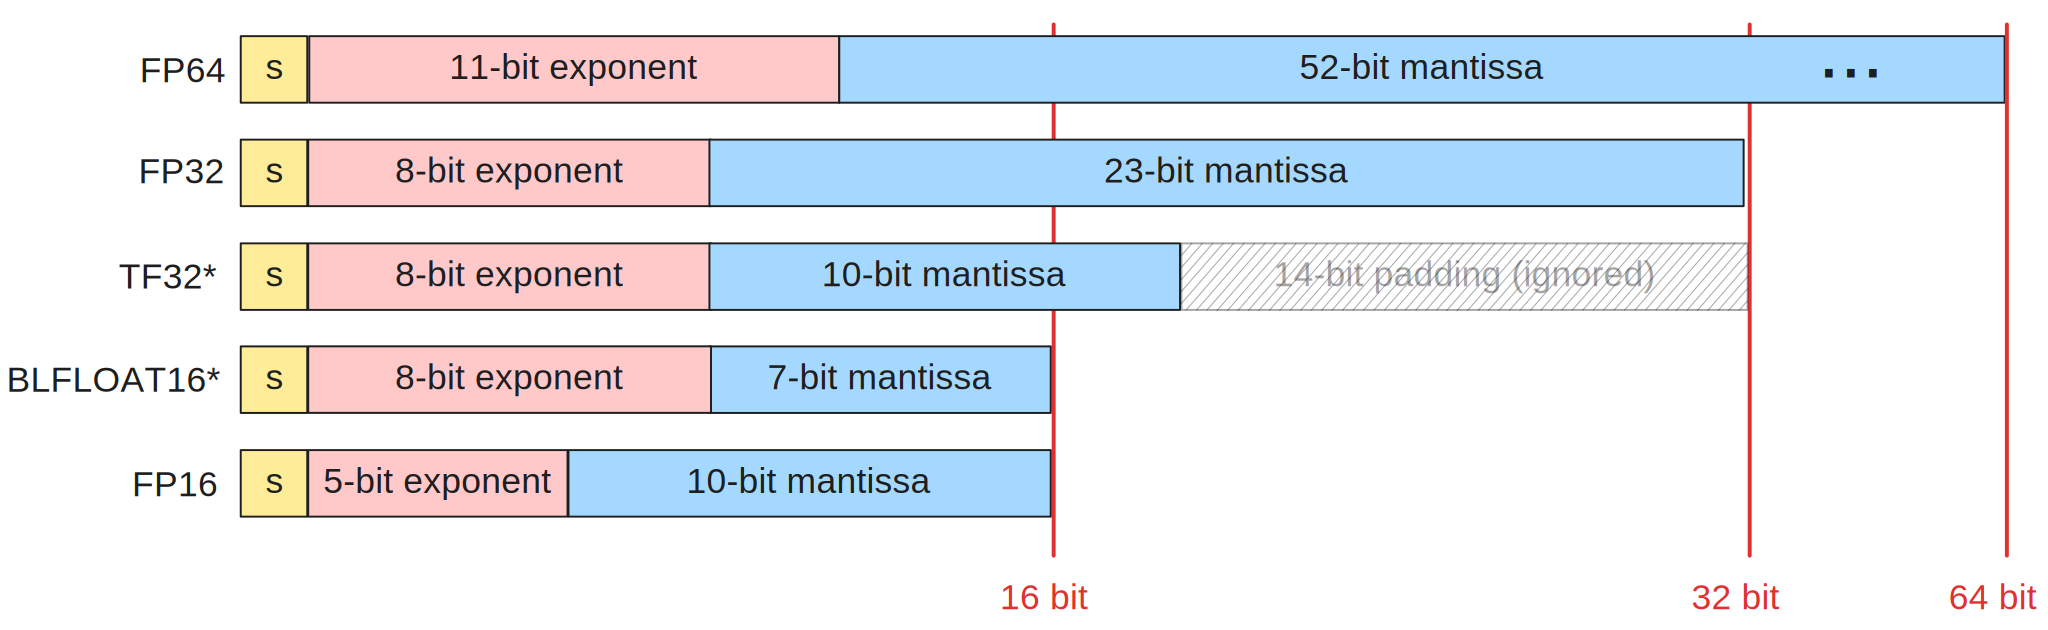
\includegraphics[width=0.9\textwidth]{FloatingPointBitComparions}
  \caption{Bit layout comparison of FP64, FP32, TF32, BF16, and FP16, with exponent and significand fields drawn to scale.}
  \label{fig:fp-bit-patterns}
\end{figure}

The number of exponent bits determines the \emph{dynamic range} (the ratio of the largest to smallest representable magnitudes), while the number of significand bits determines the \emph{precision} (the spacing between adjacent representable values). These properties are summarised in \cref{tab:fp-properties}.

\begin{table}[t]
\centering
\caption{Numerical properties of floating-point formats on the A100. Machine epsilon ($\varepsilon$) is the smallest increment to 1.0 that produces a distinct value, i.e.\ $\varepsilon = 2^{-p}$ where $p$ is the number of significand bits (including the implicit bit).}
\label{tab:fp-properties}
\begin{tabularx}{\textwidth}{l r r r}
\toprule
Format & Largest value & Smallest normal $>0$ & Machine epsilon \\
\midrule
FP64  & $\approx 1.8 \times 10^{308}$  & $\approx 2.2 \times 10^{-308}$ & $\approx 2.2 \times 10^{-16}$ \\
FP32  & $\approx 3.4 \times 10^{38}$   & $\approx 1.2 \times 10^{-38}$  & $\approx 1.2 \times 10^{-7}$  \\
TF32  & $\approx 3.4 \times 10^{38}$   & $\approx 1.2 \times 10^{-38}$  & $\approx 9.8 \times 10^{-4}$  \\
BF16  & $\approx 3.3 \times 10^{38}$   & $\approx 1.2 \times 10^{-38}$  & $\approx 7.8 \times 10^{-3}$  \\
FP16  & $65504$                         & $\approx 6.1 \times 10^{-5}$   & $\approx 9.8 \times 10^{-4}$  \\
\bottomrule
\end{tabularx}
\end{table}

Two aspects of this table merit attention. First, TF32 and BF16 share the same 8-bit exponent as FP32, so they retain the full FP32 dynamic range despite having far fewer significand bits. TF32 was introduced specifically for the Ampere tensor cores: inputs are stored as ordinary FP32 values, but the tensor core hardware internally truncates to 10 significand bits before performing the multiply-accumulate, with the accumulation itself carried out in full FP32~\cite{nvidia2020a100}. The programmer does not need to convert data explicitly; the truncation is transparent.

Second, FP16 has a severely limited dynamic range (maximum value $65504$), which makes it unsuitable for many scientific workloads without careful scaling. BF16 (``brain floating point''), originally developed for deep learning training on Google's TPUs~\cite{kalamkar2019bfloat16}, avoids this limitation by retaining the FP32 exponent range at the cost of reduced precision (7 fraction bits versus 10 for FP16).

\subsubsection{A100 Throughput by Precision}\label{sec:a100-fp-throughput}

The performance gap between precisions is substantial. \Cref{tab:a100-throughput-by-format} reproduces the A100 throughput figures from NVIDIA's Ampere optimisation guide~\cite{nvidia2020gtc-ampere}, broken down by execution unit.

\begin{table}[t]
\centering
\caption{Peak floating-point throughput (TFLOPS) of the A100 by format and execution unit. Tensor core figures in parentheses include sparsity acceleration (2:4 structured sparsity). Data from~\cite{nvidia2020gtc-ampere}.}
\label{tab:a100-throughput-by-format}
\begin{tabularx}{\textwidth}{l r r r}
\toprule
Format & Scalar (CUDA cores) & Vector (CUDA cores) & Tensor cores \\
\midrule
FP64   & \num{9.7}  & \num{9.7}  & \num{19.5} \\
FP32   & \num{19.5} & \num{19.5} & \num{156} (TF32) \\
FP16   & \num{19.5} & \num{78}   & \num{312} (\num{624}) \\
BF16   & \num{19.5} & \num{39}   & \num{312} (\num{624}) \\
\bottomrule
\end{tabularx}
\end{table}

The ratios are stark. Moving from FP64 CUDA core arithmetic (\SI{9.7}{\tera\flops}) to FP32 (\SI{19.5}{\tera\flops}) doubles throughput at no algorithmic cost. Engaging the tensor cores in TF32 mode yields a further $8\times$ increase to \SI{156}{\tera\flops}, and FP16/BF16 tensor core throughput reaches \SI{312}{\tera\flops}---a $32\times$ factor over FP64. Even accounting for the fact that many kernels are memory-bandwidth-bound rather than compute-bound, the reduced data movement from using 32-bit instead of 64-bit values halves the memory traffic, which directly benefits bandwidth-limited operations.

\subsubsection{The Case for Single Precision in Tensor Network Computations}\label{sec:fp32-argument}

The choice of FP64 in scientific software is often driven by convention rather than necessity~\cite{higham2022mixed}. Double precision provides roughly 15--16 decimal digits of accuracy, while single precision provides 7--8. Whether the additional digits matter depends on the conditioning of the computation and the accuracy actually required by the application. Higham and Mary~\cite{higham2022mixed} survey a broad class of numerical linear algebra algorithms where mixed- or reduced-precision arithmetic achieves results of comparable quality to FP64 at substantially lower cost---an observation that applies directly to the tensor contractions considered here.

For tensor network algorithms, several factors favour FP32:

\begin{enumerate}
  \item \textbf{Physical observables are approximate.} Tensor network methods are inherently approximate---the bond dimension truncation introduces controlled errors that typically far exceed single-precision rounding. When the truncation error is $\BigO(10^{-4})$ to $\BigO(10^{-6})$, carrying $10^{-16}$ precision in every floating-point operation is wasteful.
  \item \textbf{Iterative refinement.} Many tensor network algorithms are iterative (e.g.\ DMRG sweeps, variational optimisation). Rounding errors from FP32 arithmetic are corrected at each iteration, so they do not accumulate in the same way as in a single long computation.
  \item \textbf{Memory pressure.} Tensors with large bond dimensions consume substantial memory. Halving the per-element storage from 8 bytes to 4 bytes doubles the tensor sizes that fit in GPU memory, or equivalently allows larger bond dimensions for the same memory budget.
  \item \textbf{Bandwidth amplification.} Since tensor contractions are frequently memory-bandwidth-bound (\cref{sec:gpu-memory-hierarchy}), the $2\times$ reduction in data movement from FP32 translates almost directly into a $2\times$ speedup for bandwidth-limited kernels, before accounting for any compute throughput gains.
\end{enumerate}

The combination of these factors yields a practical speedup well in excess of the raw $2\times$ compute ratio, as demonstrated in the benchmarks in \cref{sec:results}. Where necessary, mixed-precision strategies---accumulating in FP32 while storing in FP16 or BF16---can push performance further (see~\cite{higham2022mixed} for a rigorous treatment), though this thesis focuses on FP32 as the primary working precision.

\subsection{Memory Hierarchy}\label{sec:gpu-memory-hierarchy}
\begin{figure}[H]
  \centering
  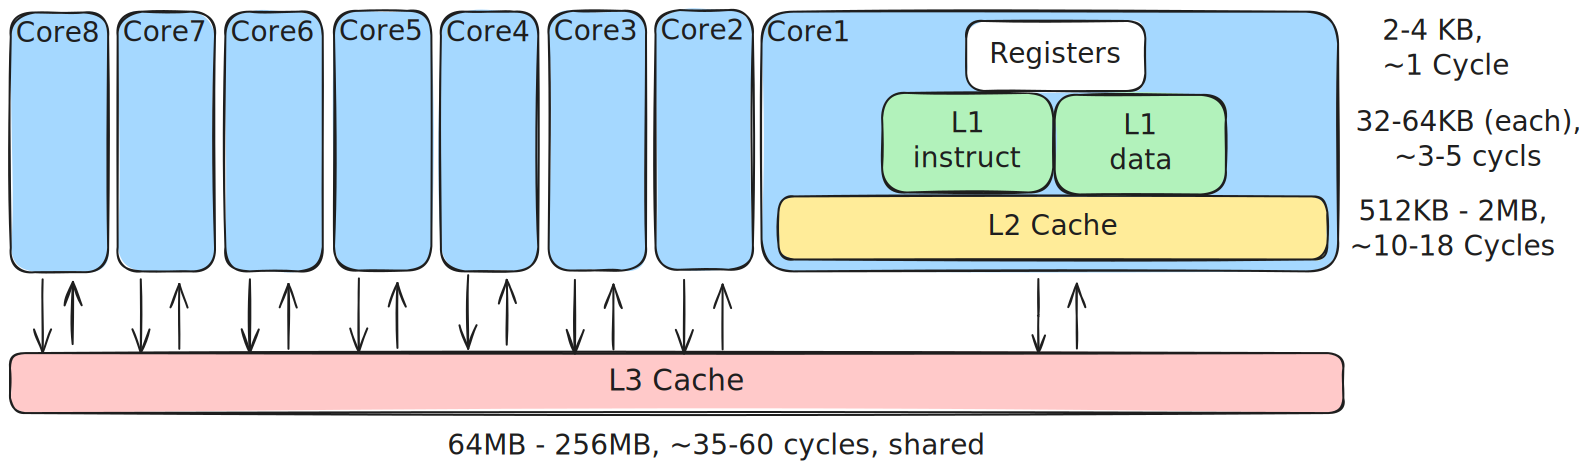
\includegraphics[width=0.9\textwidth]{CPUCacheHierarchy}
  \caption{Memory hierarchy of a modern CPU, showing the register file and cache levels (L1, L2, L3) before main memory (DRAM).}
  \label{fig:cpu-cache-hierarchy}
\end{figure}
As shown in \cref{fig:cpu-cache-hierarchy}, modern CPUs rely on a deep cache hierarchy to reduce effective memory latency.


\paragraph{GPU Memory Hierarchy}
\begin{figure}[H]
  \centering
  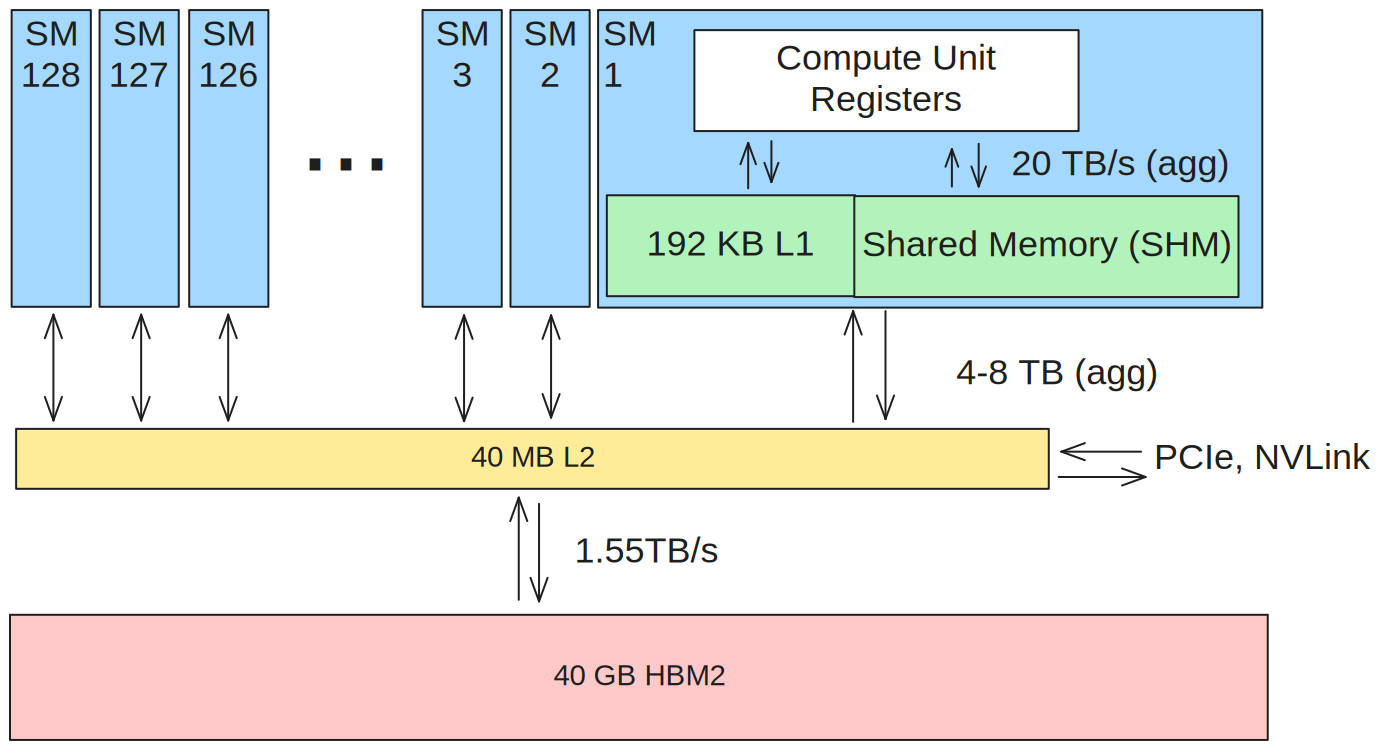
\includegraphics[width=0.65\textwidth]{A100CacheHierarchy}
  \caption{Memory hierarchy of a modern CPU, showing the register file and cache levels (L1, L2, L3) before main memory (DRAM).}
  \label{fig:a100-cache-hierarchy}
\end{figure}

Where CPUs use deep cache hierarchies to hide latency, GPUs prioritise bandwidth and expose a shallower hierarchy tuned for throughput. Four levels are relevant:

\begin{itemize}
  \item \textbf{Registers} reside in the SM and offer single-cycle access. They are private to each thread and are the scarcest on-chip resource: the number of registers a kernel uses directly limits occupancy.
  \item \textbf{Shared memory} is also on-chip but visible to all threads in a block, making it the primary mechanism for explicit data reuse and inter-thread communication. Most high-performance kernels---tiled matrix multiplications, tensor contractions---stage data through shared memory to avoid repeated global loads.
  \item \textbf{L2 cache} is shared across all SMs and transparently caches global memory traffic. On the A100 it is \SI{40}{\mega\byte}, modest relative to the core count, which reflects the throughput-oriented design.
  \item \textbf{HBM (global memory)} provides the bulk storage. The A100 uses HBM2e with \SI{80}{\giga\byte} capacity and a peak bandwidth of \SI{2039}{\giga\byte\per\second} (\cref{tab:a100-specs}), achieved through a wide interface with thousands of parallel data lines. Access latency, however, is roughly $500\times$ that of a register access (\cref{tab:a100-memory-latency}).
\end{itemize}

The practical consequence is that most scientific GPU kernels, including tensor contractions, are memory-bandwidth-bound rather than compute-bound. Performance therefore hinges on maximising reuse in registers and shared memory and accessing HBM in coalesced, bandwidth-efficient patterns.

\subsection{NVIDIA A100 Ampere Architecture}\label{sec:a100}
\subsubsection{Hardware Overview}

\begin{table}[t]
\centering
\caption{Key hardware specifications of the NVIDIA A100 (SXM4-80GB).}
\label{tab:a100-specs}
\begin{tabularx}{\textwidth}{X r}
\toprule
Property & Value \\
\midrule
Streaming Multiprocessors (SMs) & \num{108} \\
CUDA cores per SM & \num{64} \\
Tensor cores per SM & \num{4} \\
Warp schedulers per SM & \num{4} \\
Maximum threads per SM & \num{2048} \\
Maximum warps per SM & \num{64} \\
Maximum blocks per SM & \num{32} \\
Register file size per SM (32-bit registers) & \num{256000} \\
Shared memory per SM (KB) & \num{164} \\
L2 cache size (MB) & \num{40} \\
HBM memory capacity (GB) & \num{80} \\
Peak memory bandwidth (GB/s) & \num{2039} \\
Base clock frequency (GHz) & \num{1.41} \\
\bottomrule
\end{tabularx}
\end{table}

The A100 employs HBM2e as its main device memory, providing the high memory bandwidth necessary to sustain its computational throughput.

\subsubsection{Theoretical Peak Performance}

\begin{table}[t]
\centering
\caption{Theoretical peak floating-point throughput of the A100 GPU.}
\label{tab:a100-peak-performance}
\begin{tabularx}{\textwidth}{X r r}
\toprule
Precision & Peak TFLOPS & Relative speed \\
\midrule
FP64 (CUDA cores) & \num{9.7} & 1.0$\times$ \\
FP64 (Tensor cores) & \num{19.5} & 2.0$\times$ \\
FP32 & \num{19.5} & 2.0$\times$ \\
TF32 (Tensor cores) & \num{156.0} & 16.1$\times$ \\
FP16 (Tensor cores) & \num{312.0} & 32.2$\times$ \\
\bottomrule
\end{tabularx}
\end{table}


\subsubsection{Derived Performance Limits}

\begin{table}[t]
\centering
\caption{Derived theoretical limits of the A100 architecture.}
\label{tab:a100-derived}
\begin{tabularx}{\textwidth}{X r}
\toprule
Metric & Value \\
\midrule
Peak FP32 performance per SM (TFLOPS) & \num{0.18} \\
Peak FP64 performance per SM (TFLOPS) & \num{0.09} \\
Tensor core FP16 performance per SM (TFLOPS) & \num{2.89} \\
Memory bandwidth per SM (GB/s) & \num{18.88} \\
Total CUDA cores & \num{6912} \\
Total FP64 cores & \num{3456} \\
Maximum resident warps & \num{6912} \\
Maximum resident threads & \num{221184} \\
Arithmetic intensity threshold FP32 (FLOPs/byte) & \num{9.6} \\
Arithmetic intensity threshold FP64 (FLOPs/byte) & \num{4.8} \\
\bottomrule
\end{tabularx}
\end{table}


\subsubsection{Memory Latency}

\begin{table}[t]
\centering
\caption{Approximate memory access latency at different hierarchy levels.}
\label{tab:a100-memory-latency}
\begin{tabularx}{\textwidth}{X r}
\toprule
Memory level & Latency (cycles) \\
\midrule
Registers & \num{1} \\
Shared memory & \num{20} \\
L2 cache & \num{200} \\
HBM global memory & \num{500} \\
\bottomrule
\end{tabularx}
\end{table}

\subsection{Compute Node Topology}\label{sec:node-topology}

The performance of GPU-accelerated applications depends not only on the GPU itself but also on the topology of the compute node---how CPUs, GPUs, and memory are interconnected. This subsection describes the node architecture of the JURECA-DC system used throughout this thesis, which is representative of modern multi-GPU HPC nodes.

\subsubsection{CPU and NUMA Topology}

Each compute node contains two AMD EPYC 7742 processors (Rome, Zen\,2 microarchitecture), each with 64 physical cores. The chips are built from a chiplet design: each socket consists of a central I/O die (cIOD) connected to eight Core Complex Dies (CCDs). Each CCD contains two Core Complexes (CCXes), and each CCX contains four cores sharing a \SI{16}{\mega\byte} L3 cache. The hierarchy is shown in \cref{fig:numa-cpu-node}.

\begin{figure}[H]
  \centering
  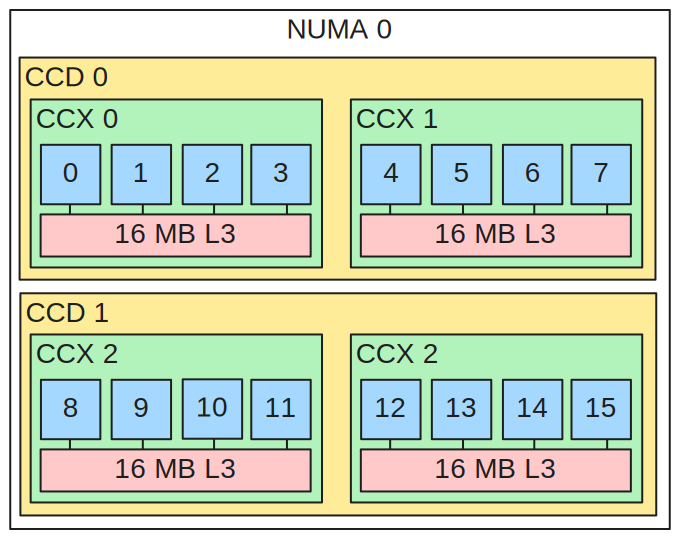
\includegraphics[width=0.5\textwidth]{NumaCPUNode}
  \caption{NUMA and chiplet hierarchy of a single AMD EPYC 7742 socket. Each socket contains 8 CCDs grouped into 4 NUMA domains (NPS=4 configuration). Each CCD holds two CCXes, each with 4 cores and a private \SI{16}{\mega\byte} L3 cache. All CCDs connect to a central I/O die that houses the memory controllers and PCIe root complexes.}
  \label{fig:numa-cpu-node}
\end{figure}

The BIOS is configured with NPS=4, which exposes four NUMA domains per socket (eight in total across the node). Each NUMA domain encompasses two CCDs (16 cores, 32 threads with SMT) and a quarter of the socket's memory controllers. This configuration allows the operating system and runtime to make NUMA-aware allocation decisions. The latency hierarchy within a socket, from fastest to slowest, is:

\begin{enumerate}
  \item \textbf{Intra-CCX:} cores sharing the same \SI{16}{\mega\byte} L3 cache communicate through it at low latency.
  \item \textbf{Intra-CCD, cross-CCX:} cores in different CCXes of the same CCD must communicate through the I/O die, as each CCX has its own independent L3.
  \item \textbf{Cross-CCD, same socket:} traffic between CCDs in different NUMA domains routes through the I/O die's internal Infinity Fabric switches.
  \item \textbf{Cross-socket:} traffic between the two sockets traverses AMD's Infinity Fabric inter-socket links (xGMI), incurring the highest latency.
\end{enumerate}

\subsubsection{GPU Interconnect Topology}

Each node has four NVIDIA A100-SXM4-40GB GPUs arranged in a fully connected mesh via NVLink\,3.0. Every GPU pair is connected by four NVLink bridges (denoted NV4 in NVIDIA's topology notation), providing \SI{100}{\giga\byte\per\second} of uni-directional bandwidth between any two devices. This symmetric, all-to-all connectivity means that multi-GPU tensor contractions do not suffer from topology-dependent bandwidth asymmetries.

Each GPU is physically attached via PCIe Gen\,4 $\times$16 to a specific NUMA domain on one of the two CPU sockets:

\begin{table}[H]
\centering
\caption{GPU-to-NUMA affinity on a JURECA-DC compute node.}
\label{tab:gpu-numa-affinity}
\begin{tabular}{l l l l}
\toprule
GPU & Socket & NUMA domain & CPU cores (physical) \\
\midrule
GPU\,0 & 0 & 3 & 48--63 \\
GPU\,1 & 0 & 1 & 16--31 \\
GPU\,2 & 1 & 7 & 112--127 \\
GPU\,3 & 1 & 5 & 80--95 \\
\bottomrule
\end{tabular}
\end{table}

The full topology, including the three classes of CPU--GPU data paths, is illustrated in \cref{fig:gpu-topology}. 

\begin{figure}[H]
  \centering
  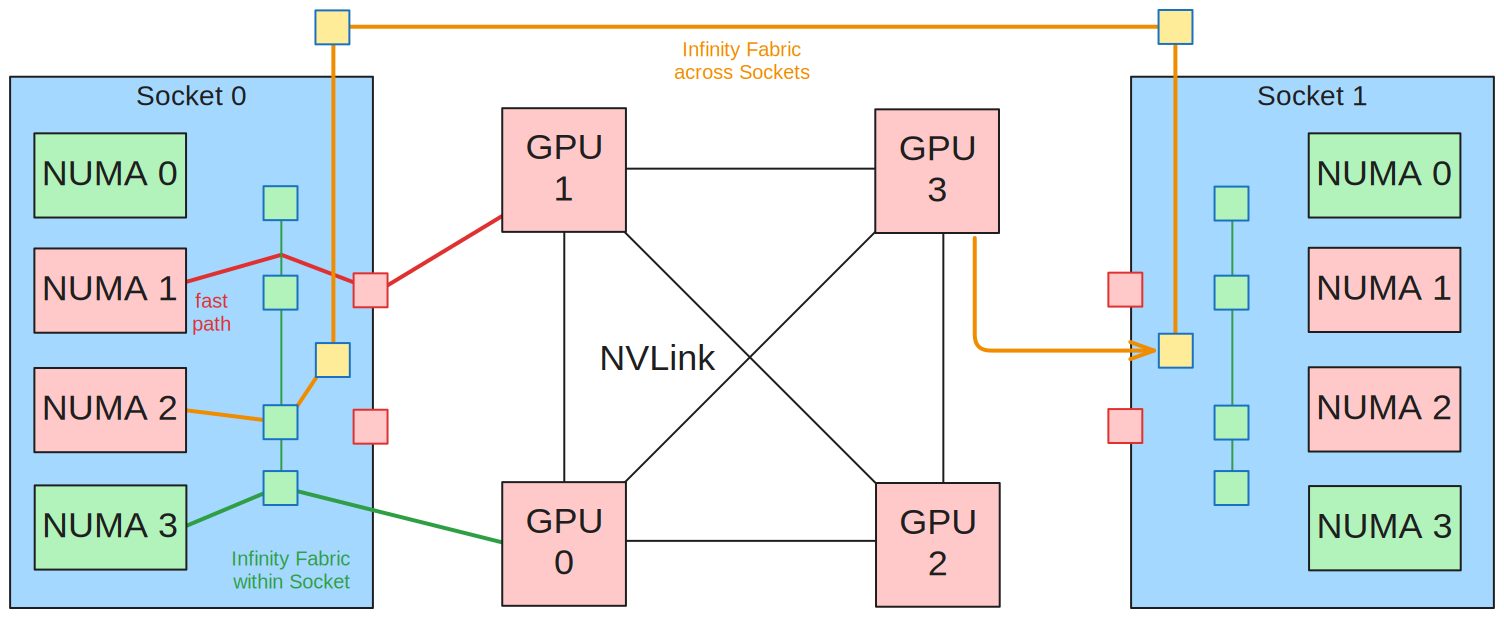
\includegraphics[width=0.9\textwidth]{GPUTopology}
  \caption{Compute node topology showing the four A100 GPUs (centre) connected via NVLink\,3.0, with the two CPU sockets on either side. Three representative host--device paths are highlighted: a fast local PCIe path (GPU\,1 $\leftrightarrow$ NUMA\,1), an intra-socket Infinity Fabric path (GPU\,0 $\leftrightarrow$ NUMA\,3), and a cross-socket Infinity Fabric path (GPU\,3 $\leftrightarrow$ NUMA\,2).}
  \label{fig:gpu-topology}
\end{figure}

The distinction between these paths matters for host--device data transfers. A \texttt{cudaMemcpy} initiated from a CPU thread pinned to a GPU's local NUMA domain takes the shortest PCIe path through the I/O die. If the source thread or memory allocation resides on the wrong NUMA domain---or worse, the wrong socket---the transfer must additionally traverse Infinity Fabric, increasing latency. For GPU-to-GPU communication, NVLink bypasses the CPU subsystem entirely, making the CPU topology irrelevant for peer-to-peer transfers.

In practice, this topology has two implications for the work in this thesis:

\begin{itemize}
  \item \textbf{Single-GPU kernels:} the CPU topology is largely invisible, since kernel launch overhead is small and tensor data resides in GPU memory throughout the computation.
  \item \textbf{Multi-GPU contractions:} data distribution and inter-GPU communication use NVLink exclusively. Host-side orchestration threads are pinned to the appropriate NUMA domain to minimise any residual host--device transfer overhead.
\end{itemize}

\section{CUDA Programming Model}\label{sec:cuda}

CUDA (Compute Unified Device Architecture) is NVIDIA's parallel programming platform for general-purpose computation on GPUs. A CUDA program consists of host code, which runs on the CPU, and \emph{kernels}, which are functions launched from the host but executed in parallel across many GPU threads. The programmer specifies the parallelism by choosing a grid of thread blocks at launch time; the hardware then schedules those blocks onto the available SMs.

\subsection{Thread Hierarchy and Kernel Launch}\label{sec:cuda-threads}

CUDA organises parallel execution into a three-level hierarchy: \emph{grids}, \emph{thread blocks} (or simply \emph{blocks}), and \emph{threads}. A kernel launch creates a single grid, which is partitioned into blocks. Each block contains a fixed number of threads that execute concurrently on the same SM and can cooperate through shared memory and synchronisation barriers. Threads in different blocks cannot synchronise with each other during kernel execution.

Both the grid and each block can be specified with up to three dimensions, which provides a natural mapping for problems defined over multidimensional arrays. The dimensions are set via the \texttt{dim3} type, and each thread identifies its position using the built-in variables \texttt{threadIdx}, \texttt{blockIdx}, \texttt{blockDim}, and \texttt{gridDim}.

\begin{figure}[H]
  \centering
  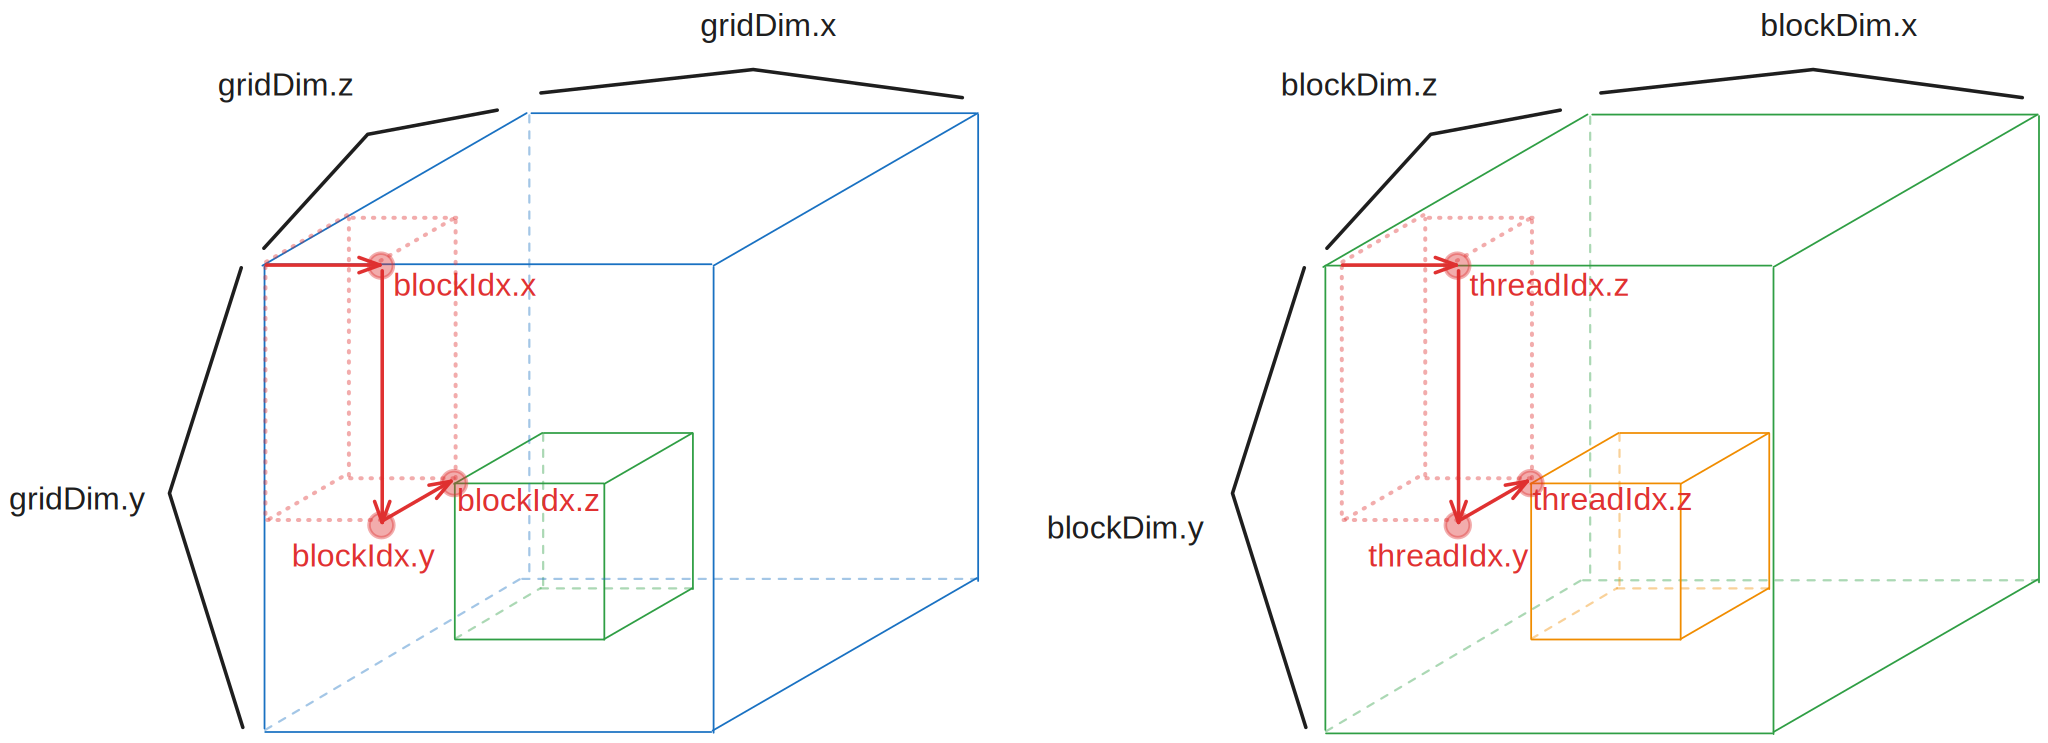
\includegraphics[width=0.85\textwidth]{GridBlockThreadAddressing}
  \caption{CUDA execution hierarchy showing the mapping of grids to thread blocks and threads. Threads are organised in up to three dimensions and identified using the built-in variables \texttt{threadIdx} and \texttt{blockIdx}.}
  \label{fig:cuda-thread-hierarchy}
\end{figure}

The hierarchical organisation of grids, thread blocks, and threads is illustrated in \cref{fig:cuda-thread-hierarchy}. Within each block, threads are further grouped into \emph{warps} of 32 threads that execute instructions in lock-step on the SM's SIMT (Single Instruction, Multiple Thread) execution units.

\subsubsection{Kernel Syntax and Launch Configuration}

A kernel is declared with the \lstinline[language=CUDA]{__global__} qualifier and launched using the triple-chevron syntax \texttt{<<<gridDim, blockDim>>>}. The following example illustrates a minimal kernel that adds two vectors element-wise:

\begin{lstlisting}[language=CUDA, caption={Element-wise vector addition kernel and its host-side launch.}, label={lst:vecadd}]
__global__ void vecAdd(const float *a, const float *b, float *c, int n) {
    int i = blockIdx.x * blockDim.x + threadIdx.x;
    if (i < n) {
        c[i] = a[i] + b[i];
    }
}

// Host launch
int n = 1 << 20;                    // 1,048,576 elements
int threadsPerBlock = 256;
int blocksPerGrid = (n + threadsPerBlock - 1) / threadsPerBlock;
vecAdd<<<blocksPerGrid, threadsPerBlock>>>(d_a, d_b, d_c, n);
\end{lstlisting}

The global thread index is computed on line~2 as \lstinline[language=CUDA]{blockIdx.x * blockDim.x + threadIdx.x}. This is the standard one-dimensional addressing pattern: \texttt{blockIdx.x} selects which block the thread belongs to, \texttt{blockDim.x} gives the number of threads per block, and \texttt{threadIdx.x} is the thread's position within its block. The bounds check on line~3 is necessary because the total number of threads launched (blocks $\times$ threads per block) is rounded up to a multiple of the block size and may therefore exceed~\texttt{n}.

\subsubsection{Two-Dimensional Grid Addressing}

For problems with a natural two-dimensional structure, such as matrix operations or image processing, both the grid and block dimensions can be specified in two (or three) dimensions. The following example demonstrates a kernel that transposes an $M \times N$ matrix:

\begin{lstlisting}[language=CUDA, caption={Matrix transpose using two-dimensional grid and block addressing.}, label={lst:transpose-2d}]
__global__ void transpose(const float *in, float *out, int M, int N) {
    int col = blockIdx.x * blockDim.x + threadIdx.x;
    int row = blockIdx.y * blockDim.y + threadIdx.y;
    if (row < M && col < N) {
        out[col * M + row] = in[row * N + col];
    }
}

// Host launch
dim3 blockDim(16, 16);          // 256 threads per block
dim3 gridDim(
    (N + blockDim.x - 1) / blockDim.x,
    (M + blockDim.y - 1) / blockDim.y
);
transpose<<<gridDim, blockDim>>>(d_in, d_out, M, N);
\end{lstlisting}

Here each thread is addressed by a \texttt{(row, col)} pair derived from the two-dimensional block and thread indices. The grid is sized so that at least $M \times N$ threads are launched, again with bounds checking to handle dimensions that are not exact multiples of the block size.

\subsubsection{Block Size Selection and Hardware Constraints}\label{sec:block-size}

The choice of block size affects both correctness and performance. The CUDA programming model imposes an upper limit of 1024 threads per block. Beyond this hard limit, several performance-relevant factors guide the choice:

\begin{itemize}
  \item \textbf{Warp granularity.} Because threads are scheduled in warps of 32, the block size should be a multiple of 32 to avoid partially filled warps whose unused lanes still consume scheduling resources.
  \item \textbf{Occupancy.} Each SM has a finite number of registers, a fixed amount of shared memory, and a maximum number of resident threads (\num{2048} on the A100). If a kernel uses many registers per thread, fewer threads can reside on the SM simultaneously, which may leave the hardware underutilised. The CUDA occupancy calculator relates block size and per-thread resource usage to the fraction of the SM's capacity that is occupied.
  \item \textbf{Shared memory per block.} Shared memory is partitioned among the blocks resident on an SM. A block that allocates a large amount of shared memory limits the number of blocks that can coexist, potentially reducing occupancy.
\end{itemize}

In practice, block sizes of 128 or 256 threads are common defaults that balance these constraints. More performance-critical kernels tune the block size empirically or use the \lstinline[language=CUDA]{__launch_bounds__} qualifier to give the compiler additional information for register allocation.

\subsubsection{Linearisation of Multidimensional Indices}\label{sec:linearisation}

GPU memory is addressed linearly, so multidimensional arrays must be mapped to one-dimensional offsets. For a tensor stored in row-major order, the linear index of element $(i, j)$ in an $M \times N$ matrix is
\begin{equation}\label{eq:row-major}
  \text{offset} = i \cdot N + j,
\end{equation}
which generalises to higher-order tensors by successive multiplication with trailing dimensions. In column-major (Fortran) order, the convention used by cuBLAS and most BLAS libraries, the index is instead
\begin{equation}\label{eq:col-major}
  \text{offset} = j \cdot M + i.
\end{equation}
\Cref{lst:transpose-2d} uses row-major layout for the input (\texttt{in[row * N + col]}) and column-major layout for the output (\texttt{out[col * M + row]}), which is precisely the transpose operation.

A concrete example: for a $4 \times 3$ matrix stored in row-major order, the element at row~2, column~1 maps to linear offset $2 \cdot 3 + 1 = 7$. Understanding this mapping is essential for implementing coalesced memory access patterns, discussed in \cref{sec:coalescing}.

\subsection{Shared Memory and Synchronisation}\label{sec:shared-memory}

Shared memory is an on-chip, programmer-managed memory space visible to all threads within a block. It serves two purposes: as a software-managed cache to stage data from global memory, and as a communication channel between threads in the same block. Because shared memory has much lower latency than global memory (approximately \num{20} cycles versus \num{500} cycles on the A100, cf.\ \cref{tab:a100-memory-latency}), its effective use is often the difference between a bandwidth-bound kernel and one that approaches peak compute throughput.

\subsubsection{Static and Dynamic Allocation}

Shared memory can be allocated statically at compile time or dynamically at launch time. Static allocation uses the \lstinline[language=CUDA]{__shared__} qualifier with a fixed array size:

\begin{lstlisting}[language=CUDA, caption={Static shared memory allocation for a tile.}, label={lst:shmem-static}]
__shared__ float tile[TILE_SIZE][TILE_SIZE];
\end{lstlisting}

Dynamic allocation is specified as a third argument in the launch configuration and accessed through an \lstinline[language=CUDA]{extern __shared__} declaration:

\begin{lstlisting}[language=CUDA, caption={Dynamic shared memory allocation.}, label={lst:shmem-dynamic}]
extern __shared__ float smem[];

// Host launch with dynamic shared memory size in bytes
kernel<<<grid, block, sharedBytes>>>(args);
\end{lstlisting}

Dynamic allocation is useful when the tile size depends on runtime parameters, which is common in autotuned kernels.

\subsubsection{Tiled Matrix Multiplication}\label{sec:tiled-matmul}

The canonical use of shared memory is tiled (or blocked) matrix multiplication. A na\"ive matrix multiplication kernel that computes $C = AB$ with $A \in \R^{M \times K}$ and $B \in \R^{K \times N}$ has each thread compute one element of $C$ by reading an entire row of $A$ and column of $B$ from global memory. This results in $\BigO(K)$ global loads per thread and an arithmetic intensity of roughly $2\;\text{FLOPs}/\text{byte}$---well below the A100's crossover point of $\approx 9.6\;\text{FLOPs}/\text{byte}$ for FP32 (\cref{tab:a100-derived}).

Tiling reduces global memory traffic by loading the input matrices into shared memory in small blocks (tiles), computing partial dot products from the tile, and then advancing to the next tile. \Cref{lst:tiled-matmul} shows the structure of this approach.

\begin{lstlisting}[language=CUDA, caption={Tiled matrix multiplication using shared memory. Each block computes one tile of the output matrix $C$.}, label={lst:tiled-matmul}]
#define TILE 16

__global__ void matmul(const float *A, const float *B, float *C,
                       int M, int N, int K) {
    __shared__ float As[TILE][TILE];
    __shared__ float Bs[TILE][TILE];

    int row = blockIdx.y * TILE + threadIdx.y;
    int col = blockIdx.x * TILE + threadIdx.x;
    float sum = 0.0f;

    for (int t = 0; t < (K + TILE - 1) / TILE; t++) {
        // Cooperative load: each thread loads one element of each tile
        int aCol = t * TILE + threadIdx.x;
        int bRow = t * TILE + threadIdx.y;
        As[threadIdx.y][threadIdx.x] = (row < M && aCol < K)
                                       ? A[row * K + aCol] : 0.0f;
        Bs[threadIdx.y][threadIdx.x] = (bRow < K && col < N)
                                       ? B[bRow * N + col] : 0.0f;

        __syncthreads();  // ensure the tile is fully loaded

        for (int k = 0; k < TILE; k++) {
            sum += As[threadIdx.y][k] * Bs[k][threadIdx.x];
        }

        __syncthreads();  // safe to overwrite tile in next iteration
    }

    if (row < M && col < N) {
        C[row * N + col] = sum;
    }
}
\end{lstlisting}

The key points of this kernel are:

\begin{enumerate}
  \item \textbf{Cooperative loading (lines 14--19).} Every thread in the block loads exactly one element of the $A$-tile and one element of the $B$-tile. The 256 threads in a $16 \times 16$ block therefore load the entire $16 \times 16$ tile cooperatively. Boundary conditions are handled by loading zero for out-of-range indices.
  \item \textbf{Barrier synchronisation (line 21).} The \lstinline[language=CUDA]{__syncthreads()} call ensures that all threads have finished writing to shared memory before any thread begins reading from the tile. A second barrier after the computation (line 27) prevents any thread from overwriting the tile before all threads have finished using it.
  \item \textbf{Data reuse.} Each element loaded into \texttt{As} is read by all 16 threads in its row; each element of \texttt{Bs} is read by all 16 threads in its column. This $16\times$ reuse from shared memory instead of global memory raises the effective arithmetic intensity by the tile size factor.
\end{enumerate}

For a tile size of $T$, the number of global memory loads per output element drops from $2K$ (na\"ive) to $2K/T$, and the arithmetic intensity increases proportionally by $T$. Larger tiles improve reuse but require more shared memory per block, which can limit occupancy.

\subsection{Memory Coalescing and Bank Conflicts}\label{sec:coalescing}

\subsubsection{Global Memory Coalescing}

When a warp executes a load or store instruction, the hardware combines the 32 individual thread addresses into as few memory transactions as possible. If consecutive threads access consecutive memory addresses (i.e.\ thread $i$ accesses address $\text{base} + i$), the accesses are \emph{coalesced} into a minimal number of 128-byte cache line transactions. Non-coalesced access patterns---strided or scattered---require multiple transactions for the same warp, wasting bandwidth.

Consider accessing a row-major $M \times N$ matrix. Iterating over columns (adjacent elements in memory) with consecutive threads produces coalesced accesses:

\begin{lstlisting}[language=CUDA, caption={Coalesced access pattern: consecutive threads read consecutive columns.}, label={lst:coalesced}]
// Coalesced: threads in a warp read adjacent elements
float val = matrix[row * N + threadIdx.x];
\end{lstlisting}

Iterating over rows with consecutive threads instead produces strided accesses with stride~$N$, which is poorly coalesced:

\begin{lstlisting}[language=CUDA, caption={Non-coalesced access pattern: consecutive threads read elements separated by stride $N$.}, label={lst:non-coalesced}]
// Non-coalesced: stride-N access
float val = matrix[threadIdx.x * N + col];
\end{lstlisting}

This distinction is particularly relevant for tensor contractions, where the choice of loop ordering and index layout determines whether the innermost memory accesses are contiguous or strided.

\subsubsection{Shared Memory Bank Conflicts}

Shared memory is divided into 32 \emph{banks}, each 4 bytes wide, interleaved in a round-robin fashion: word $k$ resides in bank $k \bmod 32$. When multiple threads in a warp access different words in the same bank simultaneously, the accesses are serialised into multiple rounds, creating a \emph{bank conflict}. The worst case is a 32-way bank conflict, where all threads hit the same bank, serialising the access entirely.

A common source of bank conflicts arises when accessing columns of a shared memory array whose leading dimension is a multiple of 32:

\begin{lstlisting}[language=CUDA, caption={Bank conflict when accessing a column of a 32-wide shared array, and the padding fix.}, label={lst:bank-conflict}]
// 32-way bank conflict: column access, stride = 32
__shared__ float tile[32][32];
float val = tile[threadIdx.x][col];  // threads 0..31 all hit same bank

// Fix: pad the leading dimension by one
__shared__ float tile[32][33];       // stride = 33, conflicts eliminated
float val = tile[threadIdx.x][col];
\end{lstlisting}

Adding one element of padding to the inner dimension changes the stride to 33, which is coprime to 32, so consecutive rows map to distinct banks. This is a standard optimisation in tiled kernels.

\subsection{Performance Profiling with Nsight Compute}\label{sec:nsight}

NVIDIA Nsight Compute is a kernel-level profiling tool for CUDA applications. It collects hardware performance counters and presents them as high-level metrics and roofline-model analyses, making it the primary tool for identifying performance bottlenecks in GPU kernels.

A typical profiling workflow proceeds as follows. First, the application is run under \texttt{ncu} (the Nsight Compute command-line interface), which replays each kernel multiple times to collect a full set of counters. Then the resulting report is examined either in the Nsight Compute GUI or by querying specific metrics from the command line.

Key metrics reported by Nsight Compute that are relevant to the optimisations discussed in subsequent chapters include:

\begin{itemize}
  \item \textbf{Achieved occupancy:} the ratio of active warps per cycle to the maximum the SM can support, indicating how effectively the kernel hides memory latency through parallelism.
  \item \textbf{Memory throughput:} the achieved bandwidth to each level of the memory hierarchy (HBM, L2, shared memory), compared against the theoretical peak. A kernel achieving close to peak HBM bandwidth is memory-bound.
  \item \textbf{Compute throughput:} the achieved FLOP/s relative to the peak, broken down by instruction type. A kernel well below peak compute with high memory throughput is bandwidth-limited.
  \item \textbf{Warp stall reasons:} a breakdown of why warps were stalled (e.g.\ waiting for memory, waiting at a barrier, instruction dependencies), which directly guides optimisation.
  \item \textbf{Shared memory bank conflicts:} the number of replayed shared memory accesses due to bank conflicts, indicating whether padding or access pattern changes are needed.
  \item \textbf{L2 cache hit rate:} the fraction of global memory requests served by the L2 cache, relevant for understanding data reuse across thread blocks.
\end{itemize}

Throughout the implementation chapters of this thesis, Nsight Compute profiles are used to validate performance models, confirm that kernels are operating in the expected regime (compute-bound or memory-bound), and guide iterative optimisation of tensor contraction kernels.

\section{Related Work}\label{sec:related-work}

\subsection{cuBLAS and cuTENSOR}\label{sec:cublas-cutensor}

\subsection{ChASE Eigensolver}\label{sec:chase}

\subsection{Existing GPU Tensor Network Implementations}\label{sec:existing-tn-gpu}
